\documentclass[12pt,a4paper,titlepage]{article}
\usepackage[utf8]{inputenc}
\usepackage{polski}
\usepackage{listings}
\usepackage{graphicx}
\usepackage{xcolor}
\usepackage{minted}
\usepackage{amsmath,latexsym}
\usepackage{caption}
\usepackage{float}
\usepackage{graphicx}
\usepackage{tikz}
\usepackage{pgfplots}
\usepackage{pgfgantt}

\usepackage[colorlinks = true,
            linkcolor = black,
            urlcolor  = blue,
            citecolor = blue,
            anchorcolor = blue]{hyperref}

\pgfplotsset{compat=1.15} 

\makeatletter
\newcommand{\linia}{\rule{\linewidth}{0.4mm}}
\renewcommand{\maketitle}{\begin{titlepage}
    \vspace*{1cm}
    \begin{center}\small
    Politechnika Wrocławska\\
    Wydział Elektroniki\\
    Programowanie Efektywnych Algorytmów
    \end{center}
    \vspace{3cm}
    \noindent\linia
    \begin{center}
      \LARGE \textsc{\@title}
         \end{center}
     \linia
    \vspace{0.5cm}
    \begin{flushright}
    \begin{minipage}{7cm}
    \textit{\small Autor:}\\
    \normalsize \textsc{\@author} \par
    \end{minipage}
    \vspace{5cm}

     {\small Poniedziałek, 11\textsuperscript{15}-13\textsuperscript{00}}\\
        Dr inż. Jarosław Rudy
     \end{flushright}
    \vspace*{\stretch{6}}
    \begin{center}
    \@date
    \end{center}
  \end{titlepage}
}
\makeatother
\author{Justyna Skalska, 225942}
\title{Problem Komiwojażera\\
(BF, B\&B, DP)}

\begin{document}
\maketitle
\tableofcontents

\newpage

\section{Wstęp}
\subsection{Cel projektu}
Celem projektu było wykonanie programu, wykorzystującego algorytmy programowania
dynamicznego (Dynamic Programming), podziału i ograniczeń (Branch \& Bound) oraz przeglądu zupełnego (Brute Force) do rozwiązania problemu komiwojażera (Travelling Salesman Problem).

\subsection{Opis problemu}
Problem komiwojażera należy do klasy problemów NP-trudnych i jest on zagadnieniem optymalizacyjnym, polegającym na znalezieniu minimalnego cyklu Hamiltona w pełnym grafie ważonym. Mówiąc prościej, rozwiązaniem problemu komiwojażera jest znalezienie najkrótszej ścieżki w grafie skierowanym, rozpoczynającej się w danym wierzchołku, odwiedzającej wszystkie wierzchołki dokładnie raz i kończącej się w wierzchołku początkowym. Ścieżka taka nazywa się optymalną trasą. Ponieważ nie ma znaczenia, gdzie zaczynamy, wierzchołek początkowy może być po prostu pierwszym wierzchołkiem w grafie. W wersji asynchronicznej, odległości pomiędzy wierzchołkami mogą dodatkowo zależeć także od kierunku przejścia pomiędzy nimi. Główną trudnością w rozwiązaniu problemu jest znacząca liczba możliwych kombinacji.

\subsection{Opis instancji}
Podczas testów wykorzystane zostały instancje zamieszczone na  \href{http://jaroslaw.mierzwa.staff.iiar.pwr.wroc.pl/pea-stud/tsp/}{stronie doktora Jarosława Mierzwy}. Każdy z plików zawiera liczbę wierzchołków grafu zamieszczoną w pierwszej linii oraz ich wagi przedstawione w postaci macierzy sąsiedztwa. Do pomiarów wykorzystano także instancje uzupełniające ze \href{https://www.iwr.uni-heidelberg.de/groups/comopt/software/TSPLIB95/}{strony TSPLIB}, które pozwalają zmierzyć czas wykonywania algorytmu dla innej liczby wierzchołków niż zamieszczone na stronie doktora Mierzwy. Pozwoliło to na wykonanie pomiarów dla każdej liczby wierzchołków z przedziału 6 -- 20.

\subsection{Specyfikacja techniczna}
\begin{itemize}
    \item Program został wykonany obiektowo w języku C++,
    \item Program akceptuje dane w postaci macierzy sąsiedztwa wczytywane z pliku,
    \item Czas wykonania algorytmów mierzony był przy wykorzystaniu biblioteki std::chrono,
    \item Do dynamicznego przechowywania danych została wykorzystana biblioteka std::vector oraz samodzielnie stworzona klasa Array.
\begin{listing}[H]
\label{code:array}
\caption{Klasa Array}
\begin{minted}[autogobble,xleftmargin=0.15\textwidth,xrightmargin=0.15\textwidth,linenos,breaklines,frame=lines,framerule=2pt,framesep=10pt]{C++}
class Array
{
    size_t size;
    int *array;
    void relocate(size_t size);
public:
    Array();
    ~Array();

    void insert(size_t position, int value);
    void insertAtBeginning(int value);
    void insertAtEnd(int value);
    int get(size_t position);
    int getBeginning();
    int getEnd();
    void remove(size_t position);
    void removeAtBeginning();
    void removeAtEnd();
    size_t find(int value);
    void display();

    size_t getSize();
    int* getArray();
    void setArray(int* array);
};
\end{minted}
\end{listing}
\end{itemize}


\section{Opis algorytmów}

\subsection{Brute Force}
\subsubsection{Opis}
Algorytm przeglądu zupełnego (ang. brute force) polega na przeanalizowaniu wszystkich możliwych przypadków przejścia oraz wybraniu tego, który przedstawia najbardziej optymalną drogę. Zaletą tego algorytmu jest pewność, że otrzymany wynik jest najlepszym możliwym rozwiązaniem problemu. Zaimplementowany został algorytm przeszukiwania w głąb wywoływany rekurencyjnie ze zmiennymi śledzącymi najkrótszą drogę i koszt.

\subsubsection{Złożoność obliczeniowa}
W najgorszym wypadku złożoność algorytmu wynosi $O(n!)$. Problemem algorytmu jest to, że trzeba sprawdzić każdą z permutacji, których liczba wynosi $(n-1)!/2$. Jego złożoność czasowa okazuje się być poważnym problemem, co w praktyce czyni ten algorytm bezużytecznym dla większych zbiorów danych.

\subsection{Branch \& Bound}
\subsubsection{Opis}
Metoda podziału i ograniczeń (ang. branch \& bound) służy do rozwiązywania problemów optymalizacyjnych. Jej działanie opiera się na analizie drzewa przestrzeni stanów. Drzewo to reprezentuje wszystkie możliwe ścieżki jakimi może pójść algorytm rozwiązując dany problem. Algorytm zaczyna w korzeniu drzewa i przechodząc w głąb do liścia konstruuje rozwiązanie przy jednoczesnym obliczaniu minimum optymalnego rozwiązania - \textit{upper bound} (poprzez metodę redukcji macierzy). Po znalezieniu pierwszej drogi zaktualizowana zostaje wartość \textit{lower bound}, dzięki czemu można wyeliminować wszystkie elementy, które posiadają wartość \textit{upper bound} większą od \textit{lower bound}. Dzięki takiemu ograniczeniu można określić, które węzły są obiecujące. W dalszej fazie algorytm przegląda tylko potomków właśnie takich węzłów. Pozwala to, razem z dobraniem odpowiedniej strategii odwiedzania wierzchołków oraz liczenia granicy, zmniejszyć ilość odwiedzonych wierzchołków i szybciej znaleźć rozwiązanie problemu.
\\\\
Minusem tego algorytmu jest duża złożoność pamięciowa, gdyż dla każdego elementu tworzymy uaktualnioną kopię macierzy kosztów przejścia pomiędzy wierzchołkami. W najgorszym przypadku odwiedzimy każdy wierzchołek, tak jak przy przeglądzie zupełnym.

\subsubsection{Złożoność obliczeniowa}
\begin{itemize}
    \item Czas działania metody bound wynosi $O(n^2)$
    \item Czas działania metody boundBranch wynosi $O(n^3)$
    \item Zapamiętanie i odtworzenie macierzy to operacja rzędu $O(n^2)$
    \item Zapamiętywanie nowego najlepszego rozwiązania w czasie $O(n)$
    \item Oznacza to, że realizacja algorytmu w obrębie jednego węzła wymaga czasu $O(n^3)$
\end{itemize}
Złożoność całego algorytmu można oszacować zatem przez $O(f(n)n^3)$, gdzie $f(n)$ jest liczbą węzłów drzewa poszukiwań odwiedzanych przez algorytm.
Liczba wykonanych obliczeń zależy od konkretnych danych wejściowych i w pesymistycznym przypadku jest wykładnicza.

\subsection{Dynamic Programming (Held-Karp)}
\subsubsection{Opis}
Programowanie dynamiczne (ang. dynamic programming) jest metodą rozwiązywania złożonych problemów, poprzez rozbicie ich na zbiór podproblemów o mniejszej złożoności, przy założeniu, że każdy podproblem rozważany jest jedynie raz, a wynik jego analizy przechowywany jest do wykorzystania w późniejszych obliczeniach. Dla problemu komiwojażera, najlepszym algorytmem wykorzystującym
tę metodę, jest algorytm Helda-Karpa. Wykorzystuje on tablicę $2^{(n-1)}$ elementową indeksowaną od zera, która wypełniana jest według algorytmu Helda-Karpa. Dzięki temu jesteśmy w stanie znaleźć minimalny koszt przejścia instancji. Indeks elementu jest również maską która mówi o miastach które zostały odwiedzone. Przykładowo dla 5 miast ostatnim indeksem jest 15, czyli 01111 - ta maska mówi o odwiedzeniu wszystkich miast poza ostatnim. Mimo 5 punktów potrzebne są nam tylko 4 bity, gdyż ostatnie miasto jest już wybrane i znajdujemy wierzchołek, który zapewni nam najmniejszy koszt podroży od ostatniego wierzchołka. W tym elemencie znajduje się lista elementów mówiących o koszcie przejścia tych wszystkich miast wraz ze wskazaniem na to który punkt był ostatnim. Wybierając najmniejszy element, na przykład 2 przechodzimy do maski 11101, gdzie powtarzamy algorytm, aż do całkowitego odtworzenia drogi (na samym początku należy pamiętać o dodaniu kosztu powrotu do ostatniego wierzchołka, by można było wybrać poprawny element).

\subsubsection{Złożoność obliczeniowa}
\begin{itemize}
    \item Złożoność czasowa wynosi $O(n^2 \ast 2n)$,
    \item Złożoność pamięciowa wynosi $O(2^n \ast n)$
\end{itemize}
\section{Pomiary}
Każdy pomiar został wykonany dziesięciokrotnie, a następnie uśredniony. 
Przedstawiona poniżej tabela zawiera czasy wykonywania poszczególnych algorytmów dla wielkości instancji w przedziale 6 -- 17.
\\\\
Pomiary dla algorytmu Brute Force nie zostały wykonane dla grafów zawierających więcej niż 13 wierzchołków, ponieważ przy tak dużych wartościach po pewnym czasie pojawiał się błąd o braku pamięci. Może to wynikać ze sposobu zaimplementowania tego algorytmu. Korzysta on ze stworzonej przeze mnie dynamicznej tablicy, klasy Array.
\\\\
Również pomiary dla metody Branch \& Bound nie zostały wykonane dla instancji o wielkości 17, ponieważ czas wykonywania tego algorytmu rośnie wykładniczo co nie pozwoliło w racjonalnym czasie go przetestować.

\begin{table}[H]
    \centering
	\label{tab:result}
	{\begin{tabular}{cccc}
		\hline
		$n$ &$t_{BruteForce} (ms) $ & $t_{Branch\&Bound} (ms)$ & $t_{HeldKarp} (ms)$\\
		\hline
        6  & 0.055621      & 0.00712        & 0.027242      \\
        7  & 0.390858      & 0.149372       & 0.056237      \\
        8  & 1.796346      & 0.241425       & 0.110755      \\
        9  & 14.000695     & 0.747505       & 0.28048       \\
        10 & 135.290226    & 1.195376       & 0.895455      \\
        11 & 1 443.38634   & 1.032556       & 2.325772      \\
        12 & 20 609.5472   & 5.945219       & 5.780313      \\
        13 & 317 092.289   & 13.401737      & 8.054559      \\
        14 & -             & 25.040358      & 17.988281     \\
        15 & -             & 51.043265      & 50.884576     \\
        16 & -             & 800 271.013    & 99.771393     \\
        17 & -             & -              & 299.113289    \\
		\hline
	\end{tabular}}
	\caption{Czasy obliczeń dla ustalonej liczby wierzchołków}
\end{table}

\newpage

\subsection{Brute Force}

\begin{figure}[H]
\centering
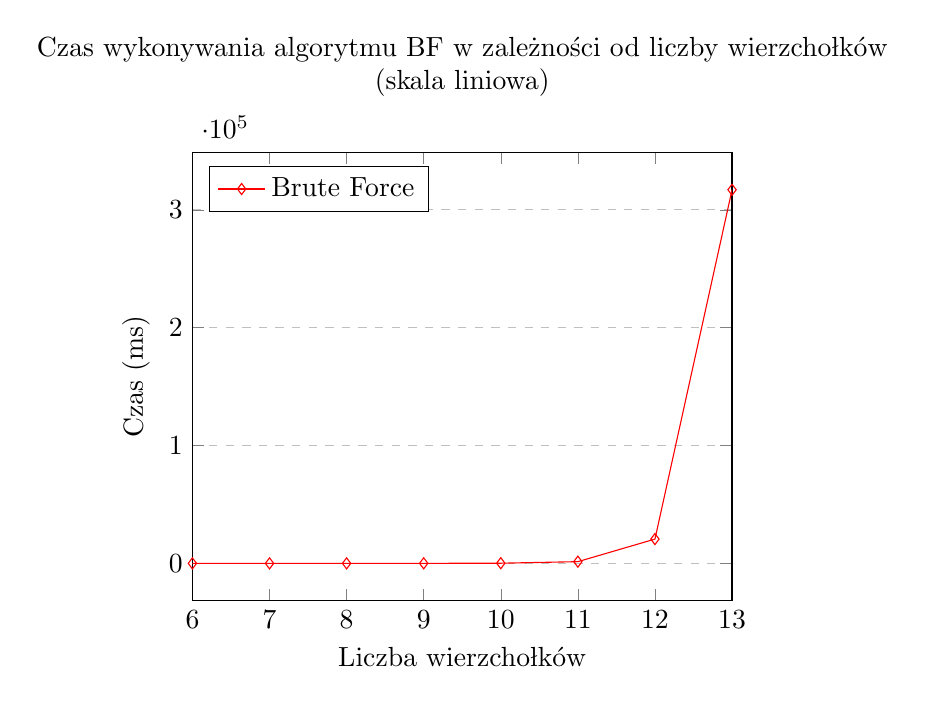
\begin{tikzpicture}
	\begin{axis}[
	    title style={yshift=2.5ex,},
	    align=center,
	    title={Czas wykonywania algorytmu BF w zależności od liczby wierzchołków\\(skala liniowa)},
		xlabel=Liczba wierzchołków,
		ylabel=Czas (ms),
        ymajorgrids=true,grid style=dashed,
        legend pos=north west,
        xmin=6,
        xmax=13
        ]
        \addplot[color=red,mark=diamond]
coordinates {
(6, 0.055621)
(7, 0.390858)
(8, 1.796346)
(9, 14.000695)
(10, 135.290226)
(11, 1 443.38634)
(12, 20 609.5472)
(13, 317 092.289)
};
\legend{Brute Force}
	\end{axis}    
\end{tikzpicture}
\end{figure}

\begin{figure}[H]
\centering
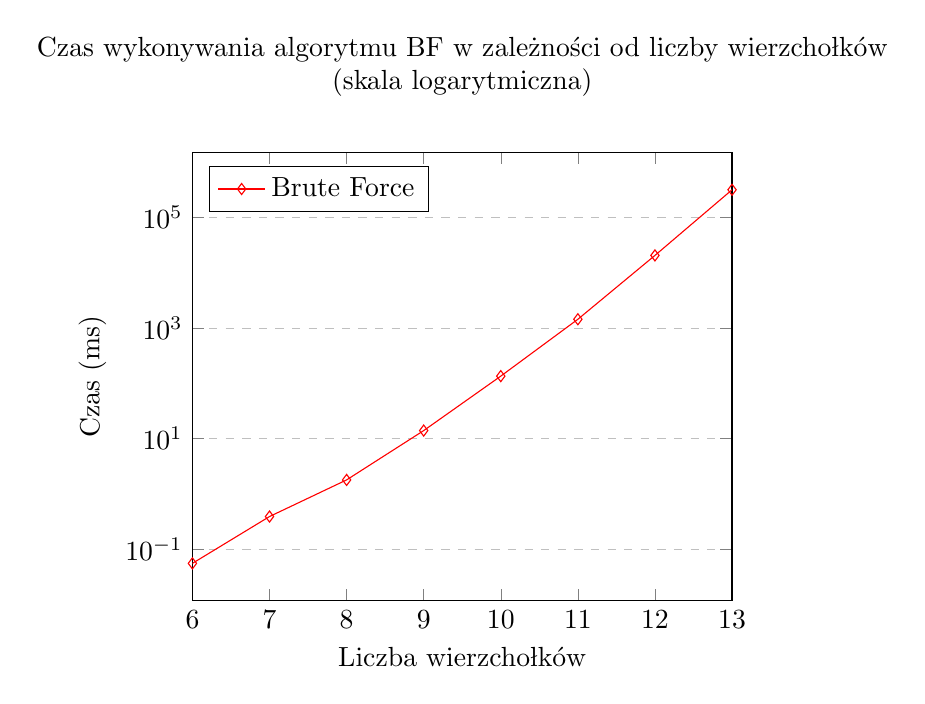
\begin{tikzpicture}
	\begin{axis}[
	    title style={yshift=2.5ex,},
	    align=center,
	    title={Czas wykonywania algorytmu BF w zależności od liczby wierzchołków\\(skala logarytmiczna)},
		xlabel=Liczba wierzchołków,
		ylabel=Czas (ms),
        ymajorgrids=true,grid style=dashed,
        legend pos=north west,
        xmin=6,
        xmax=13,
        ymode=log
        ]
        \addplot[color=red,mark=diamond]
coordinates {
(6, 0.055621)
(7, 0.390858)
(8, 1.796346)
(9, 14.000695)
(10, 135.290226)
(11, 1 443.38634)
(12, 20 609.5472)
(13, 317 092.289)
};
\legend{Brute Force}
	\end{axis}    
\end{tikzpicture}
\end{figure}

Czas wykonywanie się algorytmu dla 13 wierzchołków wynosił już około ponad 5 minut. Przy próbie wykonania go dla większej liczby po pewnym czasie pojawiał się błąd o braku pamięci. Może to wynikać ze sposobu zaimplementowania tego algorytmu.

\subsection{Branch \& Bound}

\begin{figure}[H]
\centering
\begin{tikzpicture}
	\begin{axis}[
	    title style={yshift=2.5ex,},
	    align=center,
	    title={Czas wykonywania algorytmu B\&B w zależności od liczby wierzchołków\\(skala liniowa)},
		xlabel=Liczba wierzchołków,
		ylabel=Czas (ms),
        ymajorgrids=true,grid style=dashed,
        legend pos=north west,
        ymax=150,
        xmin=6,
        xmax=16
        ]
        \addplot[color=blue,mark=square]
coordinates {
(6, 0.00712)
(7, 0.149372)
(8, 0.241425)
(9, 0.747505)
(10, 1.195376)
(11, 1.032556)
(12, 5.945219)
(13, 13.401737)
(14, 25.040358)
(15, 51.043265)
(16, 800 271.013)

};
\legend{Branch and Bound}
\end{axis}    
\end{tikzpicture}
\end{figure}

\begin{figure}[H]
\centering
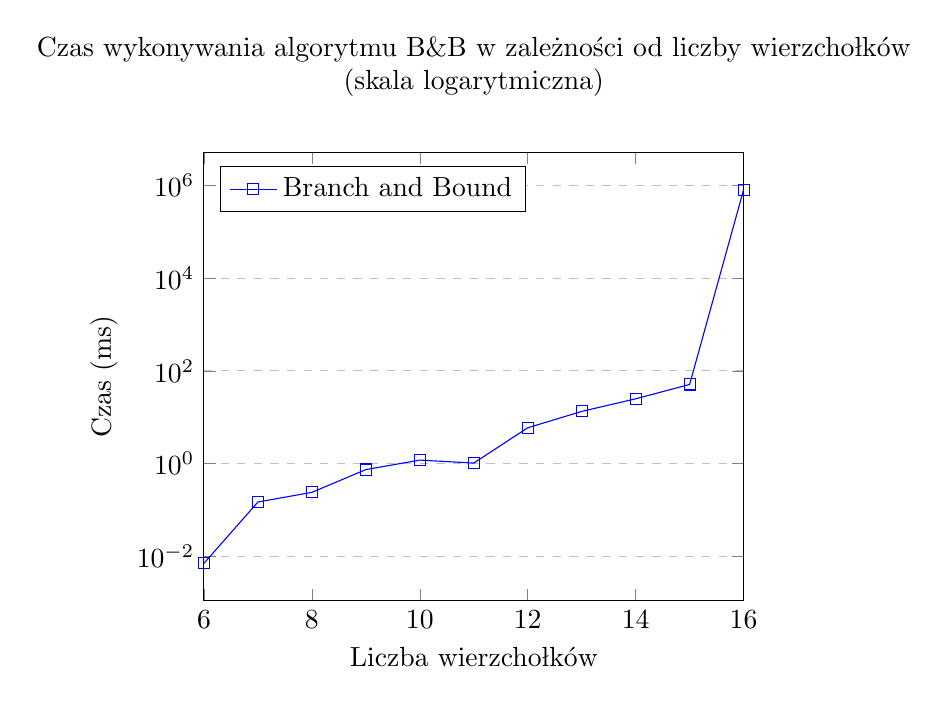
\begin{tikzpicture}
	\begin{axis}[
	    title style={yshift=2.5ex,},
	    align=center,
	    title={Czas wykonywania algorytmu B\&B w zależności od liczby wierzchołków\\(skala logarytmiczna)},
		xlabel=Liczba wierzchołków,
		ylabel=Czas (ms),
        ymajorgrids=true,grid style=dashed,
        legend pos=north west,
        xmin=6,
        xmax=16,
        ymode=log
        ]
        \addplot[color=blue,mark=square]
coordinates {
(6, 0.00712)
(7, 0.149372)
(8, 0.241425)
(9, 0.747505)
(10, 1.195376)
(11, 1.032556)
(12, 5.945219)
(13, 13.401737)
(14, 25.040358)
(15, 51.043265)
(16, 800 271.013)

};
\legend{Branch and Bound}
\end{axis}    
\end{tikzpicture}
\end{figure}

Oś czasu wykresu liniowego została ograniczona do 150ms, ponieważ czas wykonywania algorytmu dla 16 wierzchołków wynosił ponad 13 minut. Ostatnia wartość znajduje się już poza wykresem. Ograniczenie takie pozwoli zobaczyć na wykresie jak szybko rośnie czas wykonywanie algorytmu B\&B.

\subsection{Dynamic Programming (Held-Karp)}

\begin{figure}[H]
\centering
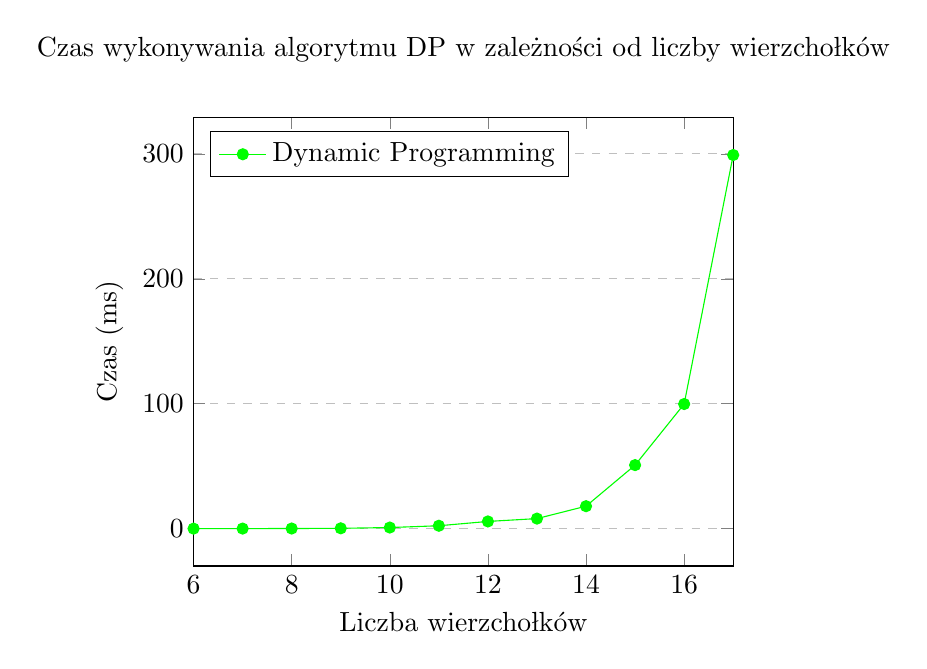
\begin{tikzpicture}
	\begin{axis}[
	    title style={yshift=2.5ex,},
	    align=center,
	    title={Czas wykonywania algorytmów w zależności od liczby wierzchołków\\(skala liniowa)},
	    title={Czas wykonywania algorytmu DP w zależności od liczby wierzchołków},
		xlabel=Liczba wierzchołków,
		ylabel=Czas (ms),
        ymajorgrids=true,grid style=dashed,
        legend pos=north west,
        xmin=6,
        xmax=17
        ]
        \addplot[color=green,mark=*]
coordinates {
(6, 0.027242)
(7, 0.056237)
(8, 0.110755)
(9, 0.28048)
(10, 0.895455)
(11, 2.325772)
(12, 5.780313)
(13, 8.054559)
(14, 17.988281)
(15, 50.884576)
(16, 99.771393)
(17, 299.113289)
};
\legend{Dynamic Programming}
	\end{axis}    
\end{tikzpicture}
\end{figure}

\begin{figure}[H]
\centering
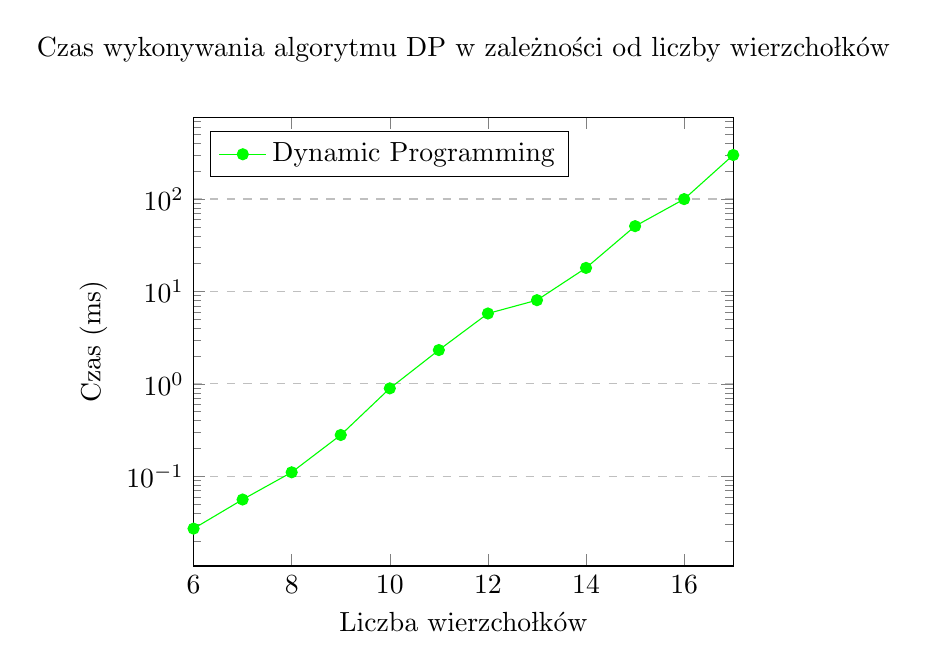
\begin{tikzpicture}
	\begin{axis}[
	    title style={yshift=2.5ex,},
	    align=center,
	    title={Czas wykonywania algorytmów w zależności od liczby wierzchołków\\(skala logarytmiczna)},
	    title={Czas wykonywania algorytmu DP w zależności od liczby wierzchołków},
		xlabel=Liczba wierzchołków,
		ylabel=Czas (ms),
        ymajorgrids=true,grid style=dashed,
        legend pos=north west,
        xmin=6,
        xmax=17,
        ymode=log
        ]
        \addplot[color=green,mark=*]
coordinates {
(6, 0.027242)
(7, 0.056237)
(8, 0.110755)
(9, 0.28048)
(10, 0.895455)
(11, 2.325772)
(12, 5.780313)
(13, 8.054559)
(14, 17.988281)
(15, 50.884576)
(16, 99.771393)
(17, 299.113289)
};
\legend{Dynamic Programming}
	\end{axis}    
\end{tikzpicture}
\end{figure}

\subsection{BF, B\&B, DP}

\begin{figure}[H]
\centering
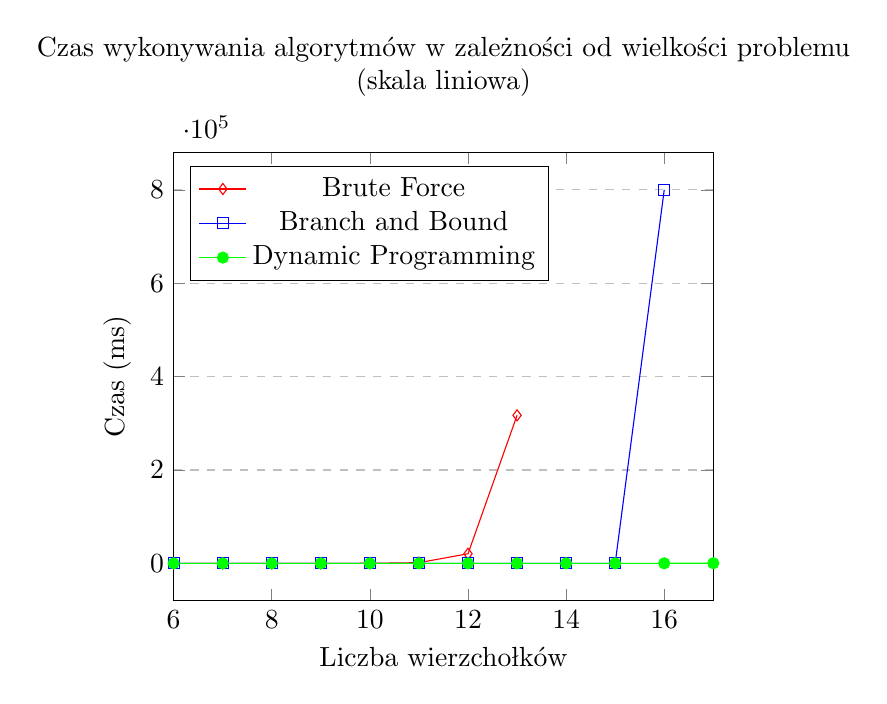
\begin{tikzpicture}
	\begin{axis}[
	    title style={yshift=2.5ex,},
	    align=center,
	    title={Czas wykonywania algorytmów w zależności od wielkości problemu \\ (skala liniowa)},
		xlabel=Liczba wierzchołków,
		ylabel=Czas (ms),
        ymajorgrids=true,grid style=dashed,
        legend pos=north west,
        xmin=6,
        xmax=17,
        ]
\addplot[color=red,mark=diamond]
coordinates {
(6, 0.055621)
(7, 0.390858)
(8, 1.796346)
(9, 14.000695)
(10, 135.290226)
(11, 1 443.38634)
(12, 20 609.5472)
(13, 317 092.289)
};

\addplot[color=blue,mark=square]
coordinates {
(6, 0.00712)
(7, 0.149372)
(8, 0.241425)
(9, 0.747505)
(10, 1.195376)
(11, 1.032556)
(12, 5.945219)
(13, 13.401737)
(14, 25.040358)
(15, 51.043265)
(16, 800 271.013)
};

\addplot[color=green,mark=*]
coordinates {
(6, 0.027242)
(7, 0.056237)
(8, 0.110755)
(9, 0.28048)
(10, 0.895455)
(11, 2.325772)
(12, 5.780313)
(13, 8.054559)
(14, 17.988281)
(15, 50.884576)
(16, 99.771393)
(17, 299.113289)
};

\legend{Brute Force,Branch and Bound, Dynamic Programming}
	\end{axis}    
\end{tikzpicture}
\end{figure}

\begin{figure}[H]
\centering
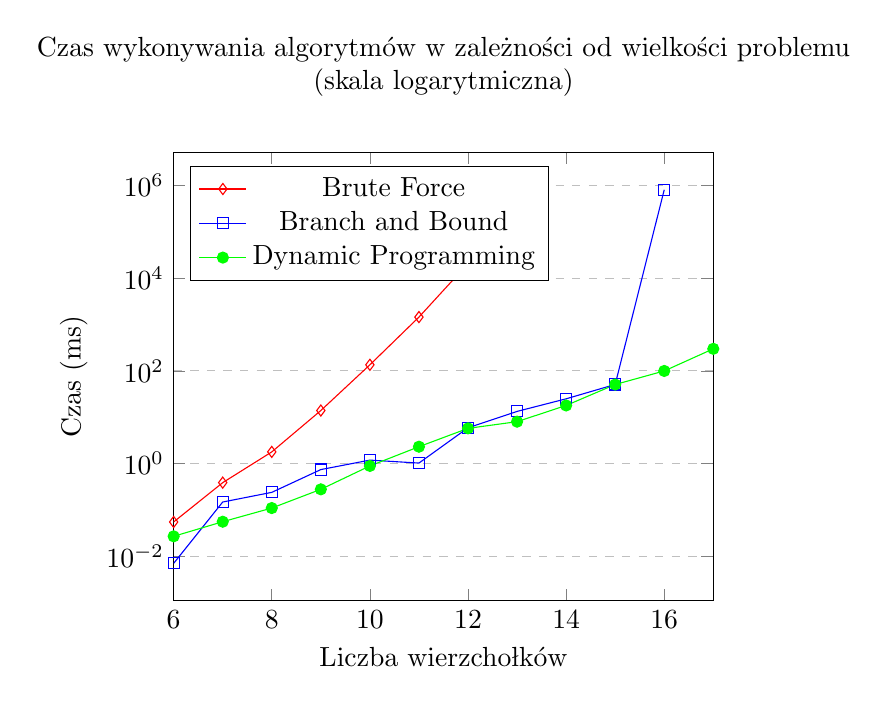
\begin{tikzpicture}
	\begin{axis}[
	    title style={yshift=2.5ex,},
	    align=center,
	    title={Czas wykonywania algorytmów w zależności od wielkości problemu \\ (skala logarytmiczna)},
		xlabel=Liczba wierzchołków,
		ylabel=Czas (ms),
        ymajorgrids=true,grid style=dashed,
        legend pos=north west,
        xmin=6,
        xmax=17,
        ymode=log
        ]
\addplot[color=red,mark=diamond]
coordinates {
(6, 0.055621)
(7, 0.390858)
(8, 1.796346)
(9, 14.000695)
(10, 135.290226)
(11, 1 443.38634)
(12, 20 609.5472)
(13, 317 092.289)
};

\addplot[color=blue,mark=square]
coordinates {
(6, 0.00712)
(7, 0.149372)
(8, 0.241425)
(9, 0.747505)
(10, 1.195376)
(11, 1.032556)
(12, 5.945219)
(13, 13.401737)
(14, 25.040358)
(15, 51.043265)
(16, 800 271.013)
};

\addplot[color=green,mark=*]
coordinates {
(6, 0.027242)
(7, 0.056237)
(8, 0.110755)
(9, 0.28048)
(10, 0.895455)
(11, 2.325772)
(12, 5.780313)
(13, 8.054559)
(14, 17.988281)
(15, 50.884576)
(16, 99.771393)
(17, 299.113289)
};

\legend{Brute Force,Branch and Bound, Dynamic Programming}
	\end{axis}    
\end{tikzpicture}
\end{figure}

\section{Wnioski}

Różnice te są tak duże, ze dokładne zaobserwowanie ich na wykresie w skali liniowej jest trudne. O wiele bardziej przydatny okazuje się wykres w skali logarytmicznej, na którym można zaobserwować jak szybko wzrasta złożoność danego algorytmu.\\\\
Jak widać algorytmy BF i B\&B stają się nieefektywne już dla dość małej liczby wierzchołków. Ponadto algorytm B\&B mimo większej wydajności zużywa dużo więcej pamięci, a jego szybkość nie jest stała - zależna od grafu jak i ilości wierzchołków grafu.\\\\
Okazuje się jednak, że dla małych instancji problemu (n $<$ 8) szybciej można sprawdzić wszystkie rozwiązania, niż wyliczać granice dla niektórych z nich i na tej podstawie podejmować decyzję o badanych rozwiązaniach. Jednakże, im większy rozmiar instancji problemu tym większa jest korzyść z wykorzystania metody podziału i ograniczeń.\\\\
Najlepszy okazał się algorytm DP, a przy okazji ma dużo mniejszą złożoność pamięciową. Algorytm ten może zostać także zoptymalizowany pamięciowo, tak aby jego złożoność była liniowa. Można to zrobić poprzez usunięcie fragmentu kodu sprawdzającego czy dany podproblem został już rozwiązany. Umożliwi to uruchomienie algorytmu DP na komputerach z mniejszą ilością pamięci. Niestety niesie to za sobą ogromny wzrost złożoności czasowej.

\end{document}